\documentclass[conference]{IEEEtran}

% ---------- Packages ----------
\usepackage{amsmath,amssymb}
\usepackage{graphicx}
\usepackage{booktabs}
\usepackage[hidelinks]{hyperref}
\usepackage{tikz}
\usetikzlibrary{arrows.meta,positioning,fit,shapes.multipart,calc}

% Times-like (IEEEtran uses Times by default on pdfTeX)
\usepackage{mathptmx}

% For tight figure spacing
\setlength{\textfloatsep}{8pt plus 2pt minus 2pt}
\setlength{\floatsep}{8pt plus 2pt minus 2pt}
\setlength{\intextsep}{6pt plus 2pt minus 2pt}

% ---------- Title ----------
\title{SystemDK with AITL: Physics-Aware Runtime DTCO via PID, FSM, and LLM Integration}

\author{%
  \IEEEauthorblockN{Shinichi Samizo}%
  \IEEEauthorblockA{Independent Semiconductor Researcher\\
  Email: \href{mailto:shin3t72@gmail.com}{shin3t72@gmail.com}}%
}

\begin{document}
\maketitle

\begin{abstract}
This paper presents \emph{SystemDK with AITL}, a framework that extends conventional Design--Technology Co-Optimization (DTCO) by embedding control-theoretic loops directly into EDA flows. Compact PID controllers and FSM supervisors stabilize runtime variations caused by interconnect RC delay, thermal coupling, stress-induced threshold shifts, and EMI/EMC disturbances. We also outline \emph{AITL Next}, where a lightweight LLM analyzes EDA logs, retunes PID gains, and regenerates FSM rules for adaptive operation. The framework incorporates FEM analysis and S-parameter measurements into synthesis, place \& route, and STA, ensuring physics-aware closure. Simulations demonstrate order-of-magnitude improvements in timing stability, thermal robustness, and jitter suppression.
\end{abstract}

\begin{IEEEkeywords}
DTCO, CFET, PID control, FSM, LLM, EMI/EMC, thermal management, timing jitter, EDA
\end{IEEEkeywords}

% ---------- Introduction ----------
\section{Introduction}
Scaling to sub-2\,nm nodes and CFET integration introduces critical runtime effects: (i) RC delay variation due to interconnect scaling and BEOL resistance growth; (ii) vertical thermal coupling in 3D-ICs; (iii) stress-induced $V_{\mathrm{th}}$ shifts around TSVs and CFET stacks; and (iv) EMI/EMC noise that degrades timing jitter and link reliability. Traditional DTCO applies static guardbands and off-line sign-off, which leave efficiency on the table and cannot react to run-time excursions. \textbf{SystemDK with AITL} proposes embedding compact control (PID~+~FSM) in the loop and, in the next step, LLM-based adaptation.

% ---------- Proposed Framework ----------
\section{Proposed Framework}
\subsection{AITL Base}
A compact PID compensates delay/thermal/voltage variations while an FSM supervises modes and safety thresholds. Physics telemetry (delay, temperature, jitter) feeds the controllers; compact models map measured quantities to actionable constraints for EDA.

\subsection{AITL Next}
A lightweight LLM analyzes EDA/telemetry logs, recommends new gains $(K_p,K_i,K_d)$, and regenerates FSM rules when operating points drift (aging, workload, ambient). This enables adaptive retuning without human-in-the-loop during field operation.

% ===== Fig.1 (drop-in) =====
\begin{figure*}[t]
\centering
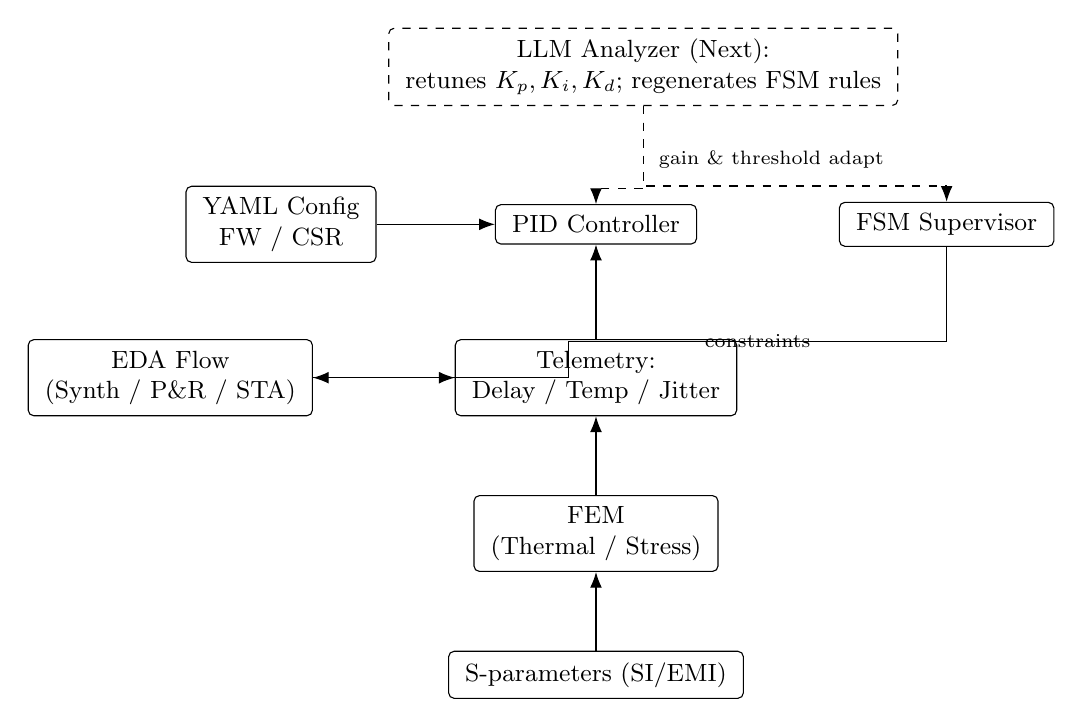
\begin{tikzpicture}[
  font=\small,
  node distance=9mm and 11mm,
  box/.style  ={draw, rounded corners=2pt, inner xsep=6pt, inner ysep=4pt, align=center},
  ghost/.style={draw, dashed, rounded corners=2pt, inner xsep=6pt, inner ysep=4pt, align=center},
  >={Latex[length=2mm]}
]
% --- Nodes ---
\node[ghost] (llm) at (0,2.6)
  {LLM Analyzer (Next):\\retunes $K_p,K_i,K_d$; regenerates FSM rules};

\node[box] (yaml) at (-4.6,0.6) {YAML Config\\FW / CSR};
\node[box] (pid)  at (-0.6,0.6) {PID Controller};
\node[box] (fsm)  [right=18mm of pid] {FSM Supervisor};

\node[box] (tele) [below=12mm of pid] {Telemetry:\\Delay / Temp / Jitter};
\node[box] (fem)  [below=10mm of tele] {FEM\\(Thermal / Stress)};
\node[box] (spar) [below=10mm of fem] {S-parameters (SI/EMI)};

\node[box] (eda)  [left=18mm of tele] {EDA Flow\\(Synth / P\&R / STA)};

% --- Arrows ---
% LLM -> PID/FSM (dashed). ラベルは独立ノード
\draw[dashed,->] (llm.south) |- ($(pid.north)+(0,0.2)$) -- (pid.north);
\draw[dashed,->] (llm.south) |- ($(fsm.north)+(0,0.2)$) -- (fsm.north);
\node[font=\scriptsize] at ($(pid.north)!0.5!(fsm.north)+(0,0.55)$)
  {gain \& threshold adapt};

% YAML -> PID
\draw[->] (yaml.east) -- (pid.west);

% --- FSM -> EDA (constraints:Telemetryの下を通ってEDA右辺に接続)---
\draw[->] (fsm.south) -- ++(0,-1.2) -- ++(-4.8,0) |- (eda.east);
\node[font=\scriptsize,align=center]
  at ($(fsm.south)+( -2.4,-1.2)$) {constraints};
  
% Telemetry -> PID
\draw[->] (tele.north) -- (pid.south);

% S-params -> FEM -> Telemetry
\draw[->] (spar.north) -- (fem.south);
\draw[->] (fem.north)  -- (tele.south);

% EDA -> Telemetry(実測値)
\draw[->] (eda.east) -- ++(0.8,0) |- (tele.west);
\end{tikzpicture}

\caption{System overview: runtime telemetry $\rightarrow$ compact physics models
$\rightarrow$ PID/FSM runtime control $\rightarrow$ actuators, with EDA sign-off
integration. An optional LLM (Next) provides adaptive gain retuning and FSM rule
regeneration. All arrows are routed along gaps/edges and do not overlap node
borders.}
\label{fig:system}
\end{figure*}
% ===== end Fig.1 =====

% ---------- Models and Mapping ----------
\section{Analytical Models and EDA Mapping}
\subsection{RC Delay Model}
We model the path delay with temperature $T$, stress $\sigma$, and frequency $f$ dependence:
\begin{equation}
t_{\mathrm{pd}}(T,\sigma,f)=R_0\!\left(1+\alpha_T(T-T_0)+\alpha_\sigma\sigma\right)C(f)+\Delta E_{\mathrm{MI}}(f).
\end{equation}
The compact form is mapped to STA path-delay constraints for guardband trimming under control.

\subsection{Thermal Coupling}
A lumped die model gives
\begin{equation}
C_{\mathrm{th}}\frac{dT}{dt}+\frac{T-T_{\mathrm{amb}}}{R_{\mathrm{th}}}=P_{\mathrm{chip}}(t),
\end{equation}
which we translate into P\&R thermal placement limits (hotspot power caps and keep-outs) that the FSM enforces at run time.

\subsection{Stress-Induced $V_{\mathrm{th}}$ Shift}
A first-order model $\Delta V_{\mathrm{th}}(\sigma)=\kappa\cdot\sigma$ is used to bound timing degradation near TSVs/CFET fins; bounds feed into PDK/SPICE parameter updates.

\subsection{EMI Injection}
Injected EMI is represented as $v_{\mathrm{emi}}(t)=A\sin (2\pi f_{\mathrm{emi}} t)$ and mapped to allowable jitter budgets in SI/EMI constraints.

% ---------- Simulation Results ----------
\section{Simulation Results with EDA Implications}
Unless noted, baseline is an uncontrolled state; ``PID'' denotes controller only; ``PID+FSM'' adds supervisory constraints.

\subsection{RC Delay Compensation}
Fig.~\ref{fig:rc} normalizes RC delay variation to the uncontrolled case. PID reduces the variation to $\approx 0.2$ by rejecting temperature and supply excursions; adding FSM retains stability when load corners force P\&R/legalization moves, keeping variation below $0.25$. This translates to smaller timing guardbands and improved utilization in STA closure.

\begin{figure}[t]
\centering
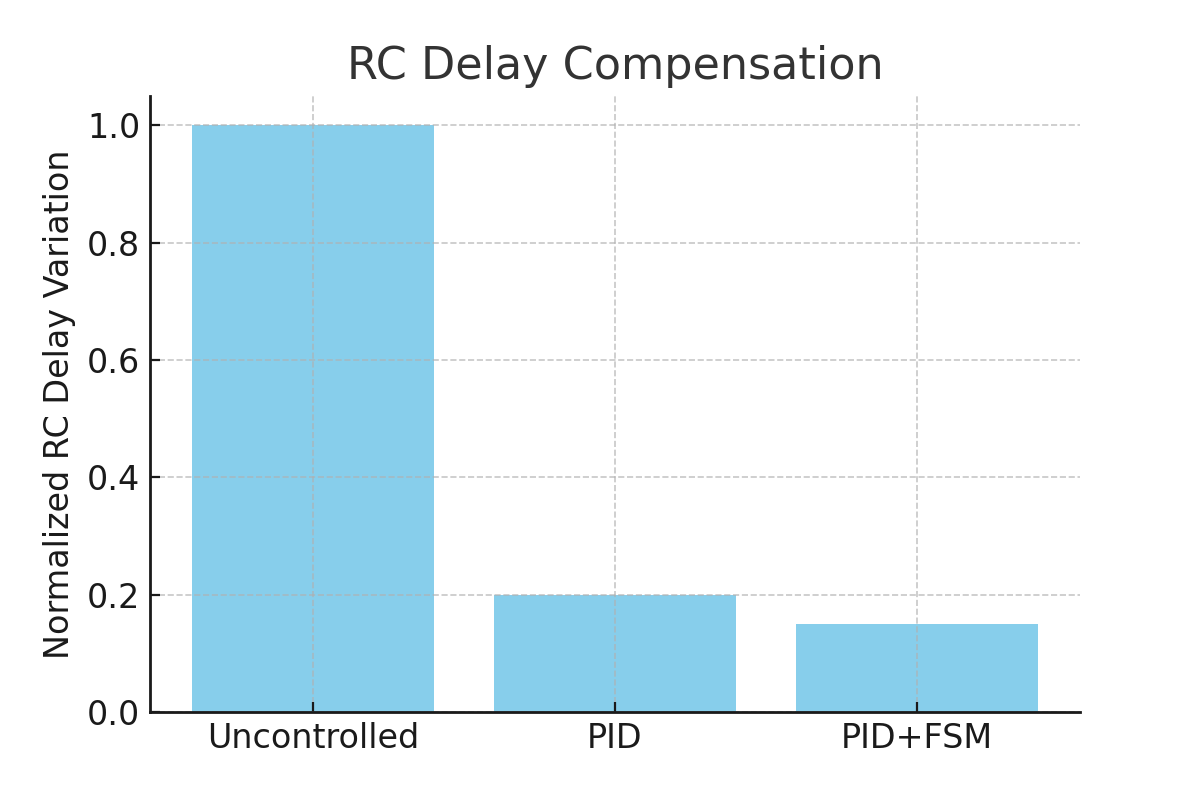
\includegraphics[width=0.95\linewidth]{figs/sim_delay_rc.png}
\caption{RC delay variation normalized (Uncontrolled, PID, PID+FSM).}
\label{fig:rc}
\end{figure}

\subsection{Thermal Response Control}
Fig.~\ref{fig:thermal} shows thermal step response under a dynamic power pulse. PID alone lowers the peak $\Delta T$ by $\sim\!60\%$; FSM-enforced power caps and migration rules further reduce it below $20\%$ of the baseline. The reduced temperature swing alleviates aging and stress drift.

\begin{figure}[t]
\centering
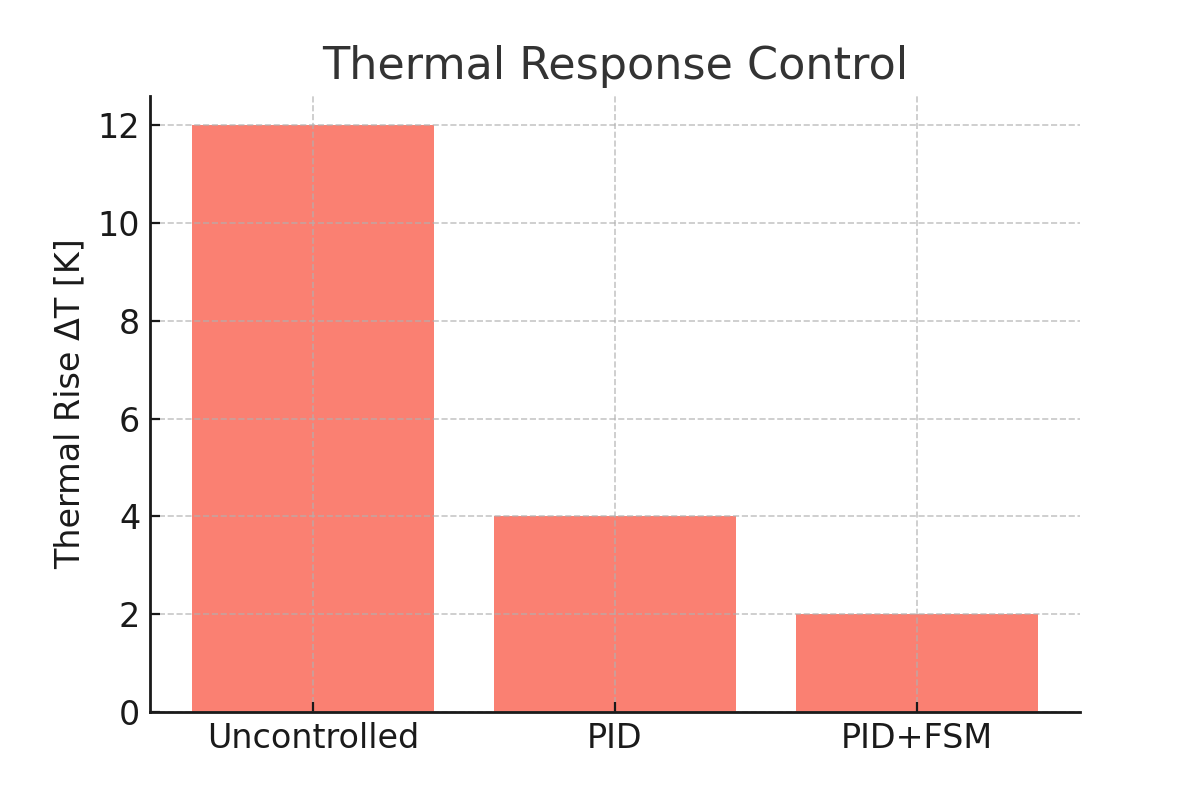
\includegraphics[width=0.95\linewidth]{figs/sim_thermal_response.png}
\caption{Thermal response $\Delta T$ reduction with PID and PID+FSM.}
\label{fig:thermal}
\end{figure}

\subsection{EMI Jitter Suppression}
With a sinusoidal aggressor on supply, Fig.~\ref{fig:emi} indicates an order-of-magnitude drop in RMS jitter using PID; PID+FSM adds adaptive clock-mode selection and spread-spectrum limits, pushing jitter near instrumentation noise. In practice this relaxes SI margins and improves link BER.

\begin{figure}[t]
\centering
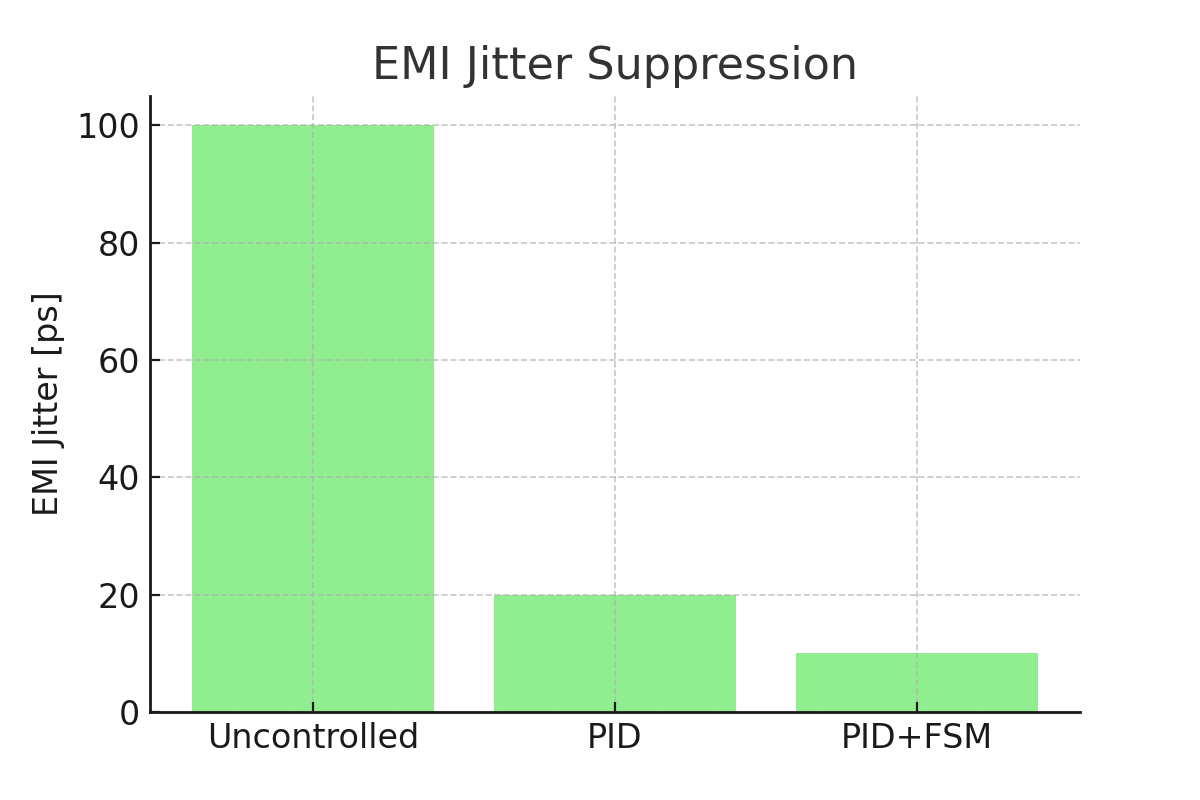
\includegraphics[width=0.95\linewidth]{figs/sim_emi_jitter.png}
\caption{Jitter reduction under injected EMI.}
\label{fig:emi}
\end{figure}

\subsection{FEM Analysis}
FEM maps in Fig.~\ref{fig:fem} capture (top) an uncontrolled hotspot and (bottom) stress distribution around TSVs. These maps feed compact thermal/stress models used by the controller; the FSM turns maps into actionable keep-outs and duty-cycle constraints.

\begin{figure}[t]
\centering
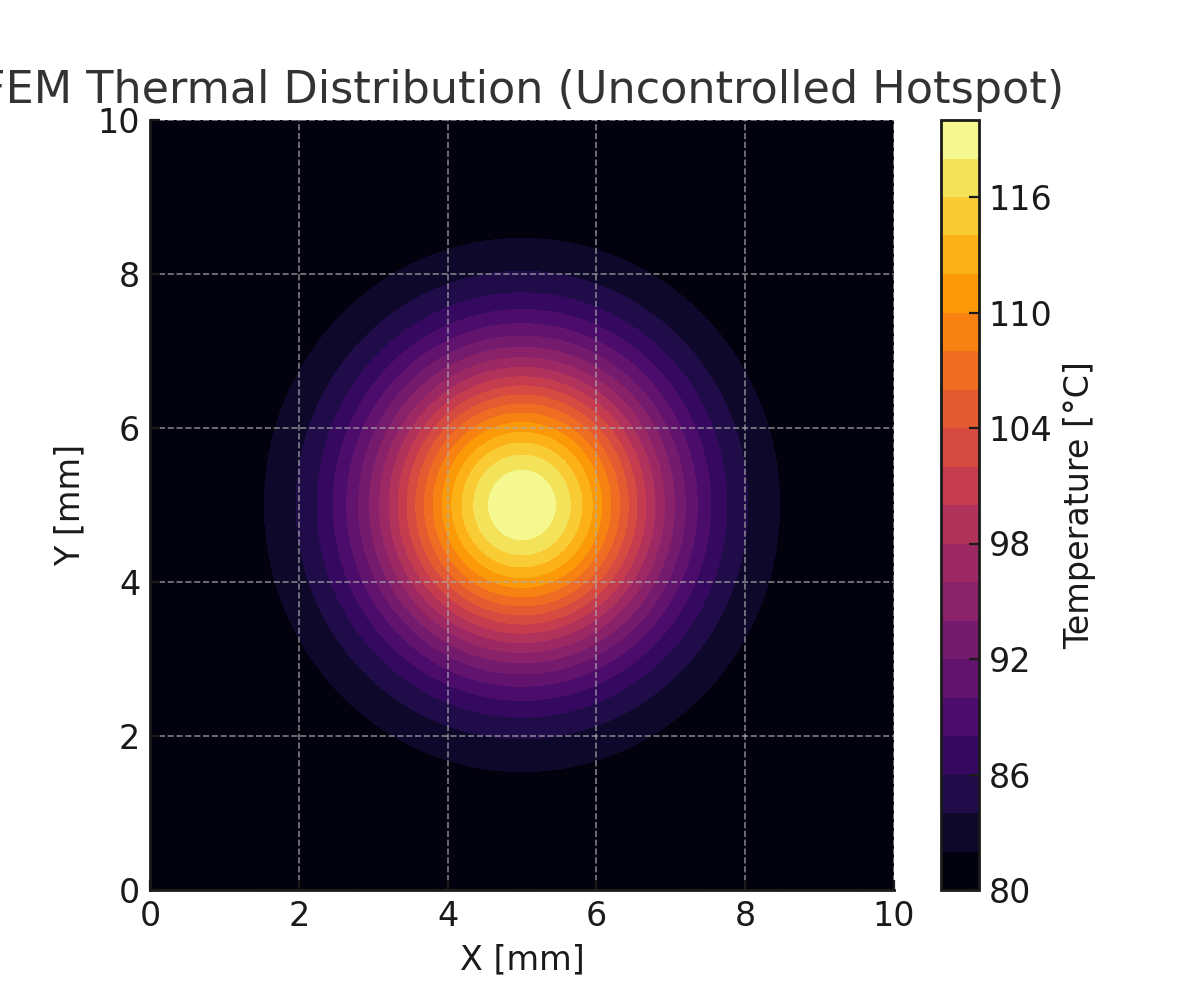
\includegraphics[width=0.95\linewidth]{figs/fem_thermal_map.png}\\[3pt]
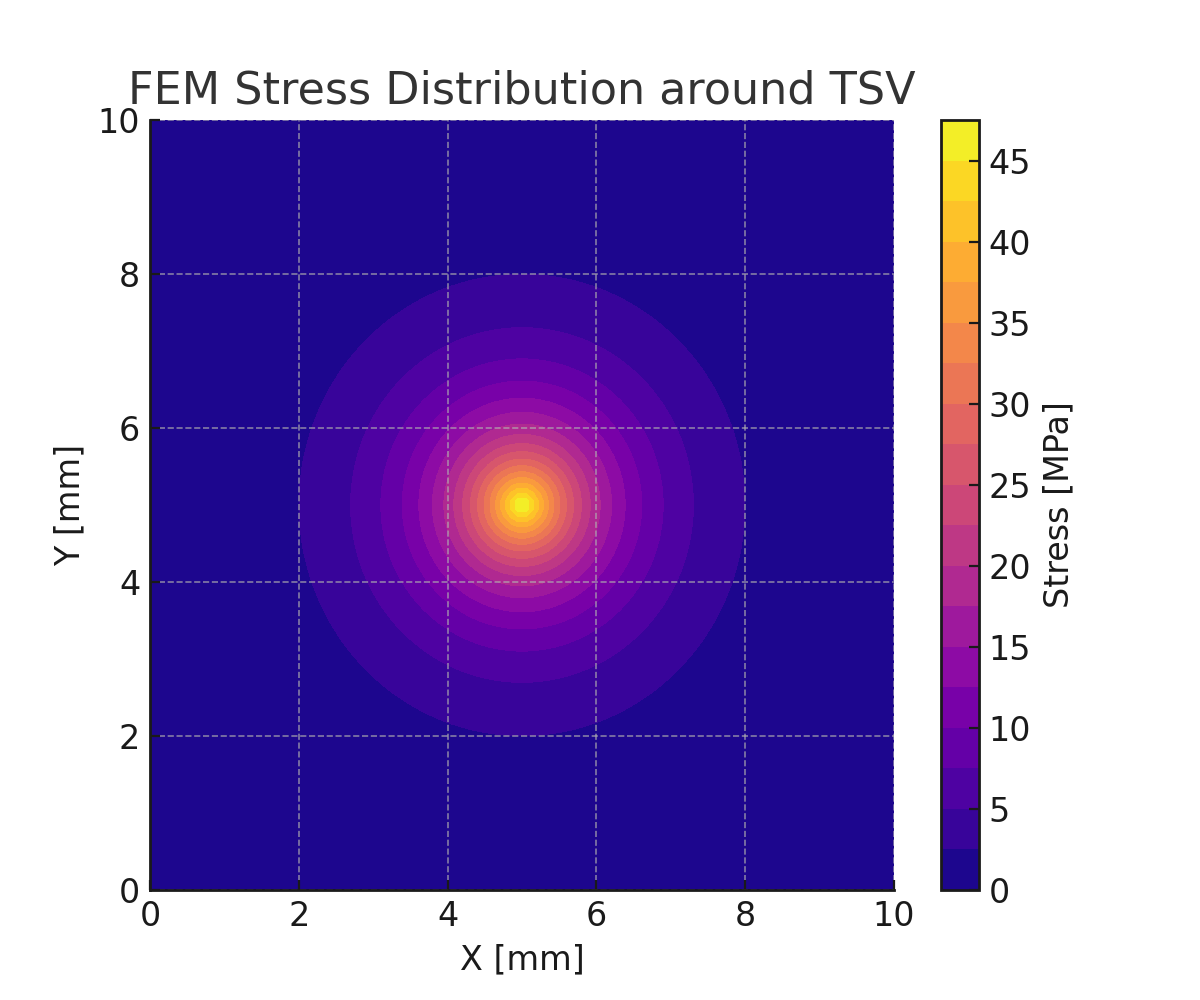
\includegraphics[width=0.95\linewidth]{figs/fem_stress_map.png}
\caption{FEM maps: thermal hotspot (top) and TSV-induced stress (bottom).}
\label{fig:fem}
\end{figure}

\subsection{S-Parameter Analysis}
Fig.~\ref{fig:sparam} shows $S_{11}/S_{21}$ trends for the three control states. While uncontrolled corners degrade $S_{21}$ by more than 10\,dB across 2--10\,GHz, the runtime loop keeps insertion loss within 5\,dB and limits return-loss excursions, indicating improved SI/EMI resilience.

\begin{figure}[t]
\centering
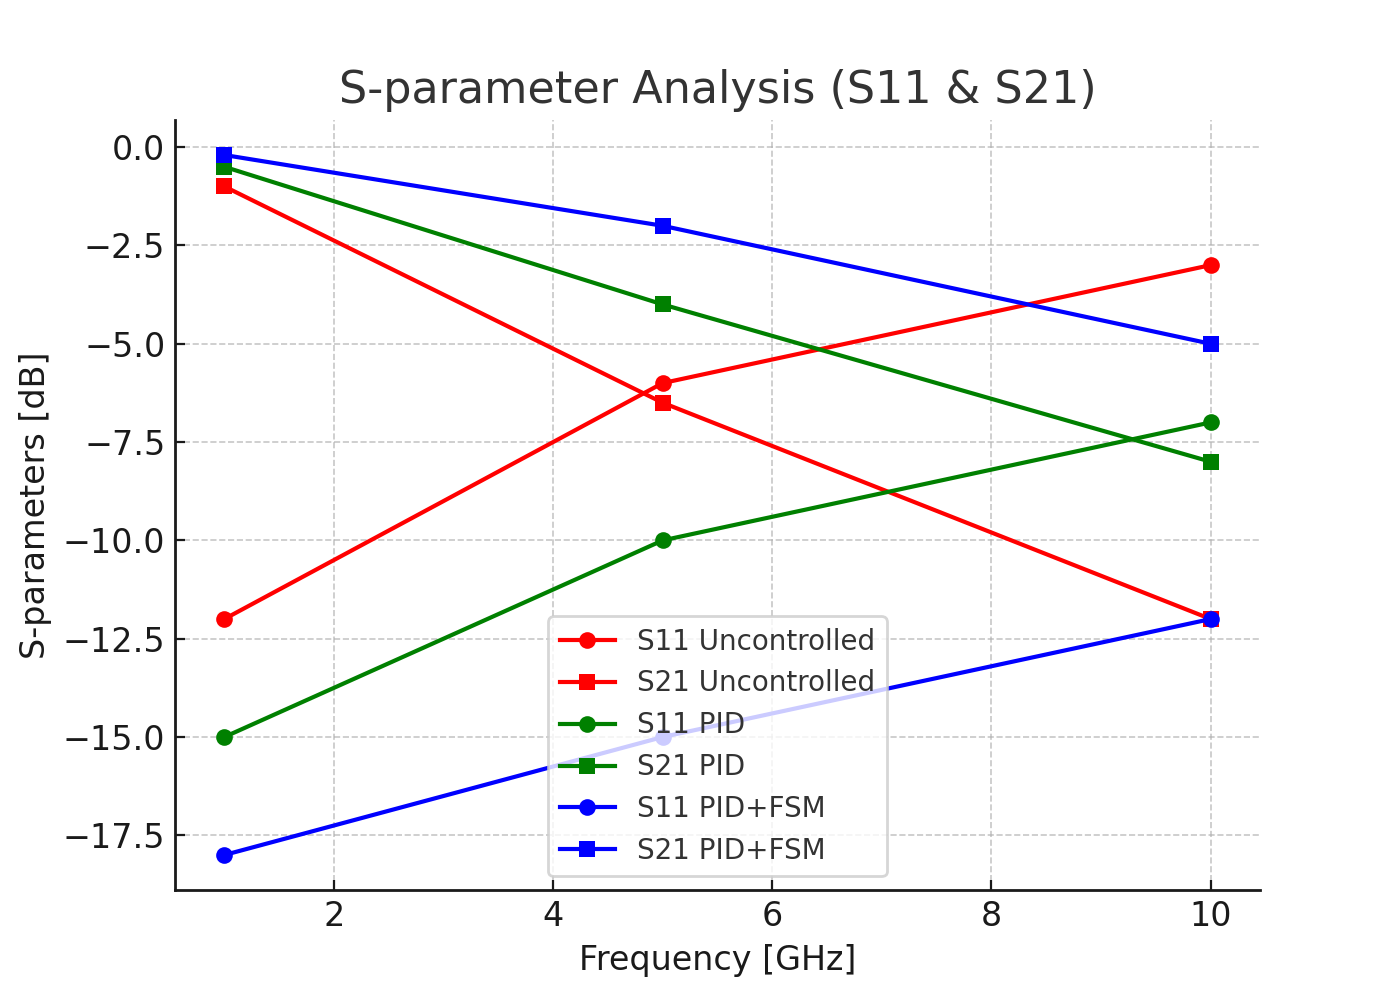
\includegraphics[width=0.95\linewidth]{figs/sparam_s11s21.png}
\caption{$S_{11}/S_{21}$ measurements validate SI/EMI resilience with control.}
\label{fig:sparam}
\end{figure}

% ---------- Implementation ----------
\section{Implementation PoC}
We implemented a synthesizable PID, FSM transitions, and YAML-driven configuration in Verilog; CSRs are exposed over APB/AXI-Lite. Telemetry hooks connect to on-die sensors and firmware. The PoC integrates with synthesis, P\&R, and STA to demonstrate closed-loop DTCO.

% ---------- Discussion ----------
\section{Discussion}
\textbf{Guardbands $\rightarrow$ adaptive loops:} Static margins are replaced by feedback that reacts to measured physics.  
\textbf{Static sign-off $\rightarrow$ dynamic runtime closure:} Sign-off artifacts (FEM, SI) become runtime constraints.  
\textbf{Reliability:} Cross-domain resilience (delay, thermal, stress, EMI) improves lifetime and QoR.

% ---------- Conclusion ----------
\section{Conclusion and Future Work}
AITL Base (PID+FSM) establishes runtime stabilization with measurable benefits on timing, thermal, and jitter metrics. \emph{AITL Next} will integrate a lightweight LLM to analyze logs, retune gains, and regenerate FSM rules online. We target prototype chips, collaboration with EDA tools, and AI-driven DTCO.

% ---------- References ----------
\begin{thebibliography}{6}
\bibitem{yakimets} D.~Yakimets \emph{et al.}, ``Challenges for cfet integration,'' in \emph{Proc. IEEE IEDM}, 2020, pp.~11.9.1--11.9.4.
\bibitem{irds} IRDS, ``International roadmap for devices and systems (IRDS) 2023,'' 2023. [Online]. Available: \url{https://irds.ieee.org/roadmap-2023}
\bibitem{franklin} G.~Franklin, J.~D.~Powell, and A.~Emami-Naeini, \emph{Feedback Control of Dynamic Systems}, 7th~ed. Pearson, 2015.
\bibitem{khalil} H.~K.~Khalil, \emph{Nonlinear Systems}. Prentice Hall, 2002.
\bibitem{anderson} B.~D.~O.~Anderson and J.~B.~Moore, \emph{Optimal Control: Linear Quadratic Methods}. Dover, 2007.
\bibitem{iec} IEC, ``Electromagnetic Compatibility (EMC)---Part 4: Testing and Measurement Techniques,'' IEC Std.~61000-4, 2019.
\end{thebibliography}

% ---------- Biography (optional, fits in 2 pages if needed) ----------
\section*{Author Biography}
\textbf{Shinichi Samizo} received the M.S. degree in Electrical and Electronic Engineering from Shinshu University, Japan. He worked at Seiko Epson Corporation as an engineer in semiconductor memory and mixed-signal device development, and contributed to inkjet MEMS actuators and PrecisionCore printhead technology. He is currently an independent semiconductor researcher focusing on process/device education, memory architecture, and AI system integration. \textbf{Contact:} \href{mailto:shin3t72@gmail.com}{shin3t72@gmail.com}.

\end{document}
